
\chapter{Ontologias}

\lettrine{A}{} palavra \textit{Ontologia} veio do grego, assim como vários outros termos que se referem à áreas de estudo. Seu significado, no entanto, é muito mais abstrato. Diferentemente de \textit{Biologia}, que é "o estudo da vida", a palavra cujo plural dá nome a esse capítulo quer dizer "o estudo do ser enquanto ser". O dicionário Merriam-Webster \cite{ontoMerriam} estende essa definição como: "um ramo da metafísica preocupado com a natureza e as relações do ser".

Importado da Filosofia, esse conceito começa a ser trabalhado muito antes da época dos computadores. Aristóteles já estudava Ontologia em suas Categorias \cite{ontoDahlberg}. No entanto, apenas em 1606, com o livro Ogdoas Scholastica, de Jacob Lorhard, foi que a palavra em si realmente surgiu. Esse termo ficou popular em 1729 com o livro Philosophia Prima sive Ontologia, de Christian Wolff, com a definição "\textit{Ontology or First Philosophy is the science of Being in general or as Being}".\cite{ontoNickles}

Para a Ciência da Computação, a definição é um pouco diferente, embora possua muita semelhança com o conceito já explícito. É estudado na área de Inteligência Artificial, que está preocupada com a automação do comportamento inteligente. Guarino \cite{ontoGuarino} definiu ontologia como "um artefato de engenharia, constituído por um vocabulário específico usado para descrever uma certa realidade, mais uma série de pressupostos explícitos acerca do significado que se atribui a esse vocabulário". Logo, uma ontologia seria uma reunião de sentenças lógicas que exibem alguma informação sobre o mundo.

Fazendo um paralelo entre ambas as disciplinas, pode-se observar que, enquanto a primeira existe um estudo sistemático da existência, na segunda existe um foco maior em o que pode ser representado.

Na prática, elas funcionam como um sistema "\textit{tell and ask}". Algumas coisas são contadas para os agentes inteligentes (uma entidade autônoma com comportamento que simula inteligência), e então, perguntas podem ser feitas para eles, embora eles não precisem saber todas as respostas. 

Surgem de um contexto onde os cientistas modelam e representar o mundo para as máquinas, e isso ocorre desde a origem dos computadores. Como cada pessoa possui uma visão de mundo, cada modelagem será diferente de algum jeito, por isso, a construção de ontologias é um tópico que merece estudo. Atualmente, a área de ontologias é bastante pesquisada por sua aplicação com Web Semântica. 

As ontologias denotam uma "especificação explícita de uma conceitualização" \cite{ontoGruber}, e, uma vez construídas, permitem comunicação, compartilhamento e reúso de conhecimentos. Elas interessam várias áreas do conhecimento, tais como a ciência da computação, filosofia, engenharia de dados, data science, lógica e linguística.

\section{Conceitualização}
	
No entanto, existe um certo debate sobre o que é uma conceitualização. Gruber \cite{ontoGruber}, que definiu o que seria uma ontologia, propôs que uma conceitualização "é uma visão abstrata e simplificada do mundo que se quer representar para algum propósito". Essa definição parece boa, mas deixa algumas pontas soltas, por exemplo, em o que seria uma "visão".

Para Guarino e Giaretta \cite{ontoGiaretta}, uma conceitualização pode ser entendida como “uma estrutura semântica intensional que codifica as regras implícitas que determinam a estrutura de uma porção da realidade”. Essa definição é um pouco mais concreta, e já é possível pensar sobre ela computacionalmente.

Pode-se inferir que uma conceitualização é uma modelagem de parte de algum domínio do conhecimento, que nada mais seria do que uma área de estudo, como a Geografia, Música, entre outros. Tal modelagem é feita a partir de alguma linguagem formal de representação (em geral, Lógicas) e deve levar em conta uma generalidade que se aplica ao domínio escolhido.

Vale lembrar que embora amplamente utilizadas, as linguagens naturais não são consideradas linguagens formais. Isso tem uma explicação simples. Uma ontologia em Português e outra em Espanhol terão vocábulos diferentes, mas podem ter a mesma conceitualização.

Debruyne \cite{ontoDebruyne} fez um estudo mais sistemático sobre o que seria uma conceitualização, baseado na pesquisa de Guarino \cite{ontoGuarino}. Para facilitar o entendimento das definições, é necessário entender dois conceitos vindos da filosofia:

\begin{itemize}
	\item Contexto Extensional: Se refere à extensão de um termo, que é o conjunto de objetos que ele denota. Um contexto é extensional se alguma expressão $ e $ aparece e pode ser substituída por uma expressão com a mesma extensão e manter o seu valor verdadeiro. No exemplo a seguir, temos que \textit{instrumento musical} é uma extensão de \textit{Violão} e de \textit{Piano}: 
	\begin{itemize}
		\item Violão é um instrumento musical.
		\item Piano é um instrumento musical.
	\end{itemize}
	
	\item Contexto Intensional: é o oposto do contexto acima. Ocorre quando um termo não pode ser substituído sem que a verdade sobre a sentença seja ameaçada. Por exemplo, embora saibamos que Clark Kent é o Super-Homem e também é um jornalista, a sentença a seguir é falsa, pois o Super-Homem não é um jornalista:
	\begin{itemize}
		\item Lois Lane acredita que o Super-Homem irá investigar uma notícia com ela. 
	\end{itemize}
	
\end{itemize}

Feita este esclarecimento, seguem as definições de Guarino.

\begin{enumerate}
	\item Noção extensional de Conceitualização: Um par $<D,R>$, onde $D$ é um domínio e $R$ são as relações relevantes que existem nesse domínio.
	\item Espaço domínio: Um par $<D,W>$, com $ D $ representando um domínio e $ W $ sendo os mundos possíveis dentro dele, ou seja, os conjuntos máximos de estados das coisas desse domínio.
	\item Relação conceitual: Dado um espaço domínio $ <D,W> $, uma relação conceitual $ \rho^n $ de aridade $ n $ em $ <D,W> $ é definida como uma função total $ \rho^n : W \to 2^{D^n}$ de W para o conjunto de todas as relações n-árias em D.
	\item Noção intensional de Conceitualização: Uma conceitualização para $ D $ é definida como uma tripla ordenada $ C=<D,W,R> $, onde $ R $ é um conjunto de relações conceituais do espaço domínio $ <D,R> $ \\ \\
	Definindo uma linguagem lógica L com um vocabulário V, teremos:
	\item Interpretação extensional de uma Linguagem: Um modelo para $ L $ é definido como uma estrutura $ <S,I> $, onde $ S=<D,R> $ é uma estrutura de mundo e $ I : V \to D \cup R $ é uma função de interpretação atribuindo elementos de D para símbolos constantes de $ V $ e elementos de $ R $ para símbolos predicados de $ V $.
	\item Interpretação intensional de uma Linguagem: Por meio de uma estrutura $ <C, I> $, onde $ C $ é uma conceitualização como definido no item 3, e $ I $ é uma função de interpretação como definido no item acima, teremos que uma interpretação intensional é um comprometimento ontológico $ K $ para $ L $. Se $ K $ é um comprometimento ontológico para $ L $, dizemos que $ L $ se compromete com $ C $ por meio de $ K $.
	\item O conjunto de modelos pretendidos de uma linguagem de acordo com um comprometimento: O conjunto $ I_K(L) $ de todos os modelos pretendidos de uma linguagem $ L $ que são compatíveis com um comprometimento $ K = <C,I> $ são todos os modelos de $ L $ que são compatíveis com $ K $. O comprometimento garante consistência.
\end{enumerate}

\section{Definições gerais (talvez diluir essa parte no capítulo)}

Smith \cite{ontoSmith} definiu alguns conceitos que nos auxiliam a compreender o que é uma ontologia.

\begin{itemize}
	\item Representação: seria uma ideia, uma imagem, um registro, ou uma descrição que se refere (ou é sobre), ou pretende referir a alguma entidade externa à representação.
	\item Representação composta: é uma representação constituída de sub-representações como suas pates, de uma maneira em que os parágrafos são feitos de sentenças e as sentenças de palavras. A menor sub-representação se chama unidade representacional, que é um ícone, um símbolo, um nome, entre outros.
	\item Representação cognitiva: é uma representação cujas unidades representacionais são ideias, pensamentos ou crenças na mente de algum elemento cognitivo.
	\item Artefato representacional: é uma representação fixa em algum meio de maneira que pode servir para fazer representações cognitivas 
	que existem nas mentes de sujeitos separados publicamente acessíveis. Exemplos: um texto, um diagrama, um mapa, uma lista, entre outros.
	\item Porção de Realidade: Termo usado que compreende universais únicos e particulares e suas combinações mais ou menos complexas.
	\item Domínio: É uma porção da realidade que forma o assunto de estudo de uma ciência ou tecnologia. Ex: Radiologia.
	\item Taxonomia: É um artefato representacional em um grafo na forma de árvore com os nós representando universais ou classes e as arestas sendo relações \textit{is-a} ou \textit{part-of}, que serão tratadas mais adiante.
	\item Ontologia: É um artefato representacional que compreende uma taxonomia própria, cujas unidades representacionais são usadas para designar uma combinação de universais, classes definidas e relações entre eles. Uma ontologia baseada em realismo é feita apenas de termos universais, para que assim ela corresponda a parte de uma teoria científica capturada pelos seus termos e interrelações.
	\item Terminologia: É um artefato representacional que possui unidades representacionais que são os termos gerais de uma linguagem para se referir a entidades em um certo domínio.
	\item Inventário: É um artefato representacional construído de termos únicos tal como nomes próprios ou identificadores alfanuméricos.
\end{itemize} 

\section{Construindo uma ontologia}

Para construir uma ontologia, é necessário escolher um domínio e o nível de generalidade que é necessário que ela atinja. Também deve-se ter em mente quem vai usá-la. Para que ela atinja o máximo de utilidade, é necessário que as perguntas que se deseja que ela responda sejam feitas antes de sua construção.

Geralmente, grandes ontologias são projetadas por equipes interdisciplinares, para que haja ela seja o mais correta e abrangente quanto possível. 

Quando se confecciona uma ontologia, é necessário que sejam feitas algumas decisões de projeto.  

Gruber \cite{ontoGruber} fez uma proposta de critérios de design para ontologias com o objetivo de tornar o compartilhamento de conhecimento e interoperabilidade com programas baseados em conhecimento mais fácil. Os critérios são os seguintes:

\begin{enumerate}
	\item Clareza: Uma ontologia deve ter uma linguagem clara e efetiva na definição de seus termos, que devem ser objetivos. Embora a definição de um conceito possa vir de situações sociais ou requisitos computacionais, ela deve ser independente destes contextos. O formalismo, no caso, o uso de uma linguagem lógica, é um meio para este fim, ou seja, quando for possível fazer uma definição usando axiomas lógicos, isso deve ser feito. Onde possível, uma definição completa (com condições necessárias e suficientes) é preferível a uma definição parcial (com condições necessárias ou suficientes). Todas devem ser documentadas usando linguagem natural.
	\item Coerência: Uma ontologia deve permitir inferências consistentes com suas definições. No mínimo, os axiomas usados nas definições devem ser logicamente consistentes. A coerência também deve ser aplicada aos conceitos informais, definidos na linguagem natural da documentação e nos exemplos. Se uma sentença que pode ser inferida contradiz uma definição ou exemplo dado informalmente, a ontologia é incoerente.
	\item Estendibilidade: Uma ontologia deve ser projetada para ser capaz de antecipar o uso de conhecimento compartilhado. Deve oferecer uma fundação conceitual de modo que o novo conhecimento possa ser apoiado nela e que a ontologia possa ser estendida e especializada, ou seja, novos termos podem ser definidos usando o vocabulário existente, de modo que a revisão do conhecimento anterior possa ser evitada ao máximo.
	\item Viés mínimo de codificação: A conceitualização deve ser especificada num nível de conhecimento que não dependa de uma codificação que utiliza um nível de símbolos particulares. Um viés de codificação ocorre quando as escolhas de representação são feitas por pura conveniência de notação ou de implementação. Isso deve ser minimizado, já que agentes de conhecimento podem ser implementados em diferentes sistemas e estilos de representação.
	\item Comprometimento ontológico mínimo: Isso faz com que ela suporte as atividades de compartilhamento de conhecimento desejadas. Deve ser feito o mínimo possível de reivindicações do mundo modelado permitindo que as partes comprometidas com a ontologia sejam livres para especializar e instanciar a ontologia o quanto quiserem. Já que isso é baseado no uso consistente do vocabulário, ele pode ser minimizado usando uma teoria fraca (genérica) e definindo apenas os conceitos necessários para a comunicação do conhecimento consistente com esta teoria.
\end{enumerate}

É possível notar que todos esses critérios não poderão ser atendidos ao mesmo tempo, portanto, alguns \textit{trade-offs} deverão ser feitos.
Podemos ter um conflito, por exemplo, entre os critérios 1 e 3, já que o máximo de clareza implica que as definições terão a sua interpretação restringida.

\subsection{Componentes de uma ontologia}

Computacionalmente falando, as ontologias possuem cinco partes. Para ilustrá-las melhor, vamos fazer uma ontologia sobre Música.

\begin{enumerate}
	\item Classes: Descrevem os conceitos de um certo domínio do discurso. São o foco das ontologias. São uma coleção de todos os particulares aos quais é possível aplicar um termo geral. Por exemplo: a classe \texttt{Cantor}.
	\item Propriedades: São atributos que descrevem características do conceito a que uma classe se refere. Em nosso exemplo, a classe Cantor possui as propriedades \texttt{Nome}, \\ \texttt{RitmoPredominante} e \texttt{Idade}.
	\item Relações: Ontologias são constituídas de relações hierárquicas. Por exemplo \texttt{Cantor} $ \to $ \texttt{Pessoa}. A hierarquia de classes representa uma relação “is-a”\cite{ontoFranca}. Tais relações são transitivas. Existem também as relações "part-of", que já estão dentro da Teoria dos Conjuntos. Uma classe é parte da outra se a compõe.
	\item Restrições: São os tipos das propriedades, por exemplo: enquanto para \texttt{Nome} e \\ \texttt{RitmoPredominante} uma \textit{string} seja suficiente, para a Idade, um inteiro já está de bom tamanho.
	\item Instância: é um indivíduo (por exemplo, \texttt{MariahCarey}), de um conjunto universal (cantores, músicos, pessoas). Vale lembrar que uma instância não é uma subclasse.
\end{enumerate}

Como já vimos acima, uma classe pode ter nomes diferentes, pois não é ele que define uma classe. Sinônimos e palavras em línguas distintas não representam classes diferentes.

Várias classes subordinadas a uma superclasse são consideradas irmãs. Elas devem ter o mesmo nível de generalidade. Por exemplo, seja uma classe Musica. Suas subclasses podem ser \texttt{Cancao} e \texttt{MusicaAmericana}, e não \texttt{Cancao}, \texttt{MusicaAmericana} e \texttt{MusicaBrasileira} (a última é sub-classe da penúltima).

Os conceitos definidos até aqui mostram um jeito de caracterizar ontologias, que é pelo número de termos que ela possui. Uma outra métrica é o número de axiomas lógicos que ela possui. 

Existem três processos para definir as classes e a hierarquia, a seguir:

\begin{itemize}
	\item \textit{Top-down}: vai das classes mais genéricas para as mais específicas.
	\item \text{Bottom-up}: vai das mais específicas indo para as mais genéricas, agrupando as específicas já criadas. 
	\item Vai-e-Vem: define conceitos simples para generalizá-los e especificá-los. Seria um misto dos dois primeiros itens.
\end{itemize}

\subsection{Montando a ontologia}

Montar uma ontologia é um processo que segue os seguintes passos:

\begin{itemize}
	\item Definir as classes da ontologia.
	\item Colocá-las em uma hierarquia taxonômica.
	\item Determinar propriedades e restrições para elas.
	\item Criar uma base de conhecimento para essas classes e propriedades, ou seja, preenchendo a ontologia com as instâncias.
	\item Colocar os valores das propriedades para as instâncias.
\end{itemize}

Embora pareça ser direto, esse processo é iterativo, como afirmam Noy e McGuinness \cite{ontoNoy}. Uma vez feito, deve ser repetido para que haja uma adequação das classes com as instâncias colocadas, pois, por exemplo, se uma classe acabar com apenas uma sub-classe, a modelagem pode ter um problema, ou a ontologia não está completa. E ainda, se uma classe possui mais de uma dúzia de sub-classes, novas categorias (classes ou subclasses) podem ser necessárias. 

Introduzir uma classe é legal quando se tem muitas propriedades específicas em muitas instâncias, o que as faz serem relacionadas de algum jeito. Se os diferentes valores nas propriedades de uma classe tornam-se muito restritos, então, uma nova classe deve ser criada para que a distinção aconteça.

O processo é iterativo, e teoricamente, ele nunca acaba. Na prática, o processo é encerrado quando a ontologia fornece respostas suficientemente boas para a maior parte das consultas realizadas, ou seja, tal critério é subjetivo.

A criação de uma ontologia é feita por uma equipe interdisciplinar, geralmente composta por \textit{experts} da área que se deseja cobrir e técnicos para a confecção de ontologias (vindos da área de Computação). Isso não limita a equipe de possuir profissionais de mais áreas.

Em relação às classes, algumas observações podem ser feitas. A primeira é em relação à herança múltipla. Ela acontece quando uma classe é sub-classe de várias outras classes, por exemplo, a classe \texttt{PopBrasileiro}, pode pertencer à classe \texttt{Pop} e à classe \texttt{MusicaBrasileira}. Isso é aceitável, pois no mundo real, acontece várias vezes e de diversas maneiras.

Outro aspecto interessante é o de classe abstrata. Uma classe desse tipo não pode ter instâncias. Em nossa ontologia, podemos ter locais (no caso, países onde as músicas são criadas). A classe \texttt{Pais} pode ter varias sub-classes, tais como \texttt{Argentina}, \texttt{Brasil}, \texttt{Portugal}, entre outras. Note que essas classes são abstratas, pois no mundo real, não existe mais de um país que possa pertencer ao conceito \texttt{Brasil}.

As ontologias possuem suporte a classes disjuntas. Classes disjuntas são aquelas que não possuem uma intersecção. Enquanto em nossa ontologia, \texttt{Cantor} e \texttt{Compositor} não sejam disjuntas. No entanto, \texttt{Cancao} e \texttt{HinoNacional} são classes disjuntas.

Uma ontologia não precisa ter toda a informação existente sobre o domínio. Não é necessário especializar ou generalizar mais do que seja necessário para a aplicação. Além disso, as classes não precisam ter todas as propriedades possíveis e nem carregarem todas as distinções que estão no mundo. Isso significa que a ontologia deve ser o modelo mais simples para o problema que se deseja resolver.

Algumas relações podem ter uma inversa, assim como ocorre com funções matemáticas. Uma relação que possui uma inversa pode ser:

\begin{itemize}
	\item \texttt{Cantor canta Musica}
	\item \texttt{Musica cantadaPor Cantor}
\end{itemize}

Para os nomes das classes, não há uma convenção específica, só há um consenso em manter um padrão de nomenclatura, por exemplo, usando \texttt{snake\textunderscore case}, \texttt{camelCase} ou usando espaços, e também prestando atenção se no nome de uma classe possui o nome de sua superclasse ou não.

\section{Usabilidade de uma ontologia}

É possível achar os usuários de uma ontologia, mas nem sempre o seu autor. O razoável é assumir que elas foram evoluindo com o passar do tempo. 

Ontologias feitas sobre áreas de estudo (por exemplo, a Aviação) serão muito mais úteis do que aquelas feitas sobre acontecimentos (queda do voo TAM 3054), cuja existência não faz sentido, já que o problema relacionado ao acontecimento pode ser resolvido usando a área de estudo relacionada.

\section{Problemas relacionados}

	Existem alguns problemas relacionados a ontologias. Os mais comuns são os problemas de modelagem e construção. Um problema muito comum é a existência, na linguagem natural, de Homônimos e Sinônimos. Deve existir um cuidado especial com eles.
	
	Em relação à modelagem, o problema de não utilizar uma equipe interdisciplinar especializada pode levar a uma cobertura incompatível de conceitos, ou seja, as classes ficam muito distantes da realidade. Além disso, usar fontes não confiáveis na ontologia pode fazer com que os problemas que elas estavam sendo feitas para resolver, não sejam resolvidos corretamente.
	
	Tais problemas tornam-se muito maiores quando duas ontologias são integradas. A possível integração entre ontologias é um dos motivos para elas existirem, afinal, isso pode acelerar o seu desenvolvimento. Em nosso exemplo, se já existir uma ontologia sobre Música Brasileira, poderemos absorvê-la, mas o cuidado terá de ser redobrado em relação às questões acima. 
	
	Em relação à implementação, os pontos que surgem são em geral a respeito da linguagem utilizada, mas isso será tratado no capítulo.
	
	Além dos já citados, pode acontecer de chegar um novo conhecimento e a ontologia ficar inconsistente. Neste caso, terão de ser usadas algumas operações de Revisão de Crenças, foco do capítulo {\color{red} X}.
	
	A ontologia construída nesse capítulo fica assim: 
	\begin{center}
		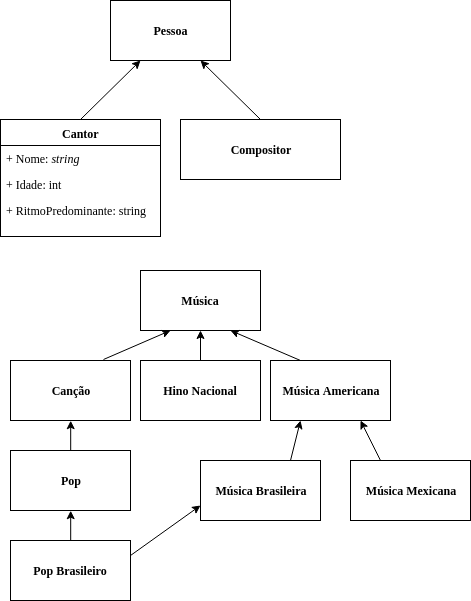
\includegraphics[width=10cm]{Capitulos/Ontologias/OntologiaMusica.png}
	\end{center}
	